From the given information, the desired equation is
\begin{align}
\norm{\vec{x}-\myvec{-3\\2}}^2 = 4^2
\\
\implies \vec{x}^T\vec{x}+\myvec{6&-4}\vec{x} -3 &=0
\end{align}
The python code for Fig. \ref{fig:4.1.1_circle} is
\begin{lstlisting}
solutions/1/codes/circle/circle1.py
\end{lstlisting}
\begin{figure}[!ht]
\centering
\includegraphics[width=\columnwidth]{./solutions/1/figs/circle/circle1.eps}
\caption{Circle using python}
\label{fig:4.1.1_circle}
\end{figure}

